\section{Datenvorverarbeitung}
\label{dv}
Wie in den Grundlagen der Datenvorverarbeitung (vgl. \vref{aufbereitung}) begründet, ist diese Phase von besonderer Bedeutung für die Güte der \gls{dm}-Resultat. Es gilt die Qualität der zuvor lediglich selektierten Zieldaten durch den Einsatz von geeigneten Verfahren nachhaltig zu verbessern und diese in einem für die \gls{dm}-Methode passendes Format bereitzustellen. Dazu müssen im Folgenden die Daten (in Form der selektierten Schüsse) zunächst von Fehlern bereinigt (siehe Data Cleaning \vref{datac}), anschließend fehlerfrei mit allen anderen verfügbaren Spiele zusammengeführt (siehe Data Integration \vref{datai})) und schließlich auf eine verwertbare Datenmenge reduziert werden (siehe Data Reduction \vref{datar}).

\subsection{Data Cleaning}
Das Data Cleaning beschäftigt sich mit den Problemarten der fehlenden, verrauschten und inkonsistenten Daten (vgl. \vref{dc}), welche nachfolgend näher untersucht und behandelt werden. 

\paragraph{Fehlende Daten}
Das ein ganzes Event, wie in diesem Falle ein Schuss, überhaupt nicht erfasst wurde, ist sehr unwahrscheinlich, da Opta als markführender Datenprovider großen Wert auf Akkuratesse und Vollständigkeit legt. Für eine exakte Überprüfung müssten über 90.000 Spielminuten (\textit{34 Spieltage x 3,5 Saisons x 9 Spiele pro Spieltag x 90 Minuten} darauf händisch geprüft werden, was zu einem nicht realisierbaren Vorgang führt. Fehlen \glqq lediglich\grqq einzelne Attribute in einem Datensatz, wie beispielsweise die x-Koordinate des Schusses, können diese Datensätze auf unterschiedliche Weise behandelt werden (siehe \vref{dc}). 



\paragraph{verrauschte Daten und Ausreißer}
Outlier-Detection $\rightarrow$ Stoppelkamp Tor\seFootcite{Vgl.}{}{DeutscherFuballBund.2014}
\paragraph{inkonsistente Daten}
Behandlung fehlerhafter Daten (z.B. $x>100$)

\paragraph{Das weiße Linienproblem}
	
\subsection{Data Integration}
\label{datai}
	\begin{itemize}
	\item Konkatenieren aller Spiele
	\item Einheitliches Format
	\end{itemize}
	
\subsection{Data Reduction}
\label{datar}
	\begin{itemize}
	\item Irrelevante Attribute entfernen
	\item Unterscheidung zwischen Tor(1) und Nicht-Tor(0)
	\item Ziel: \{"x":\_, "y":\_, "goal":\_\}
	\end{itemize}
	

\begin{sidewaysfigure}[H]
\centering
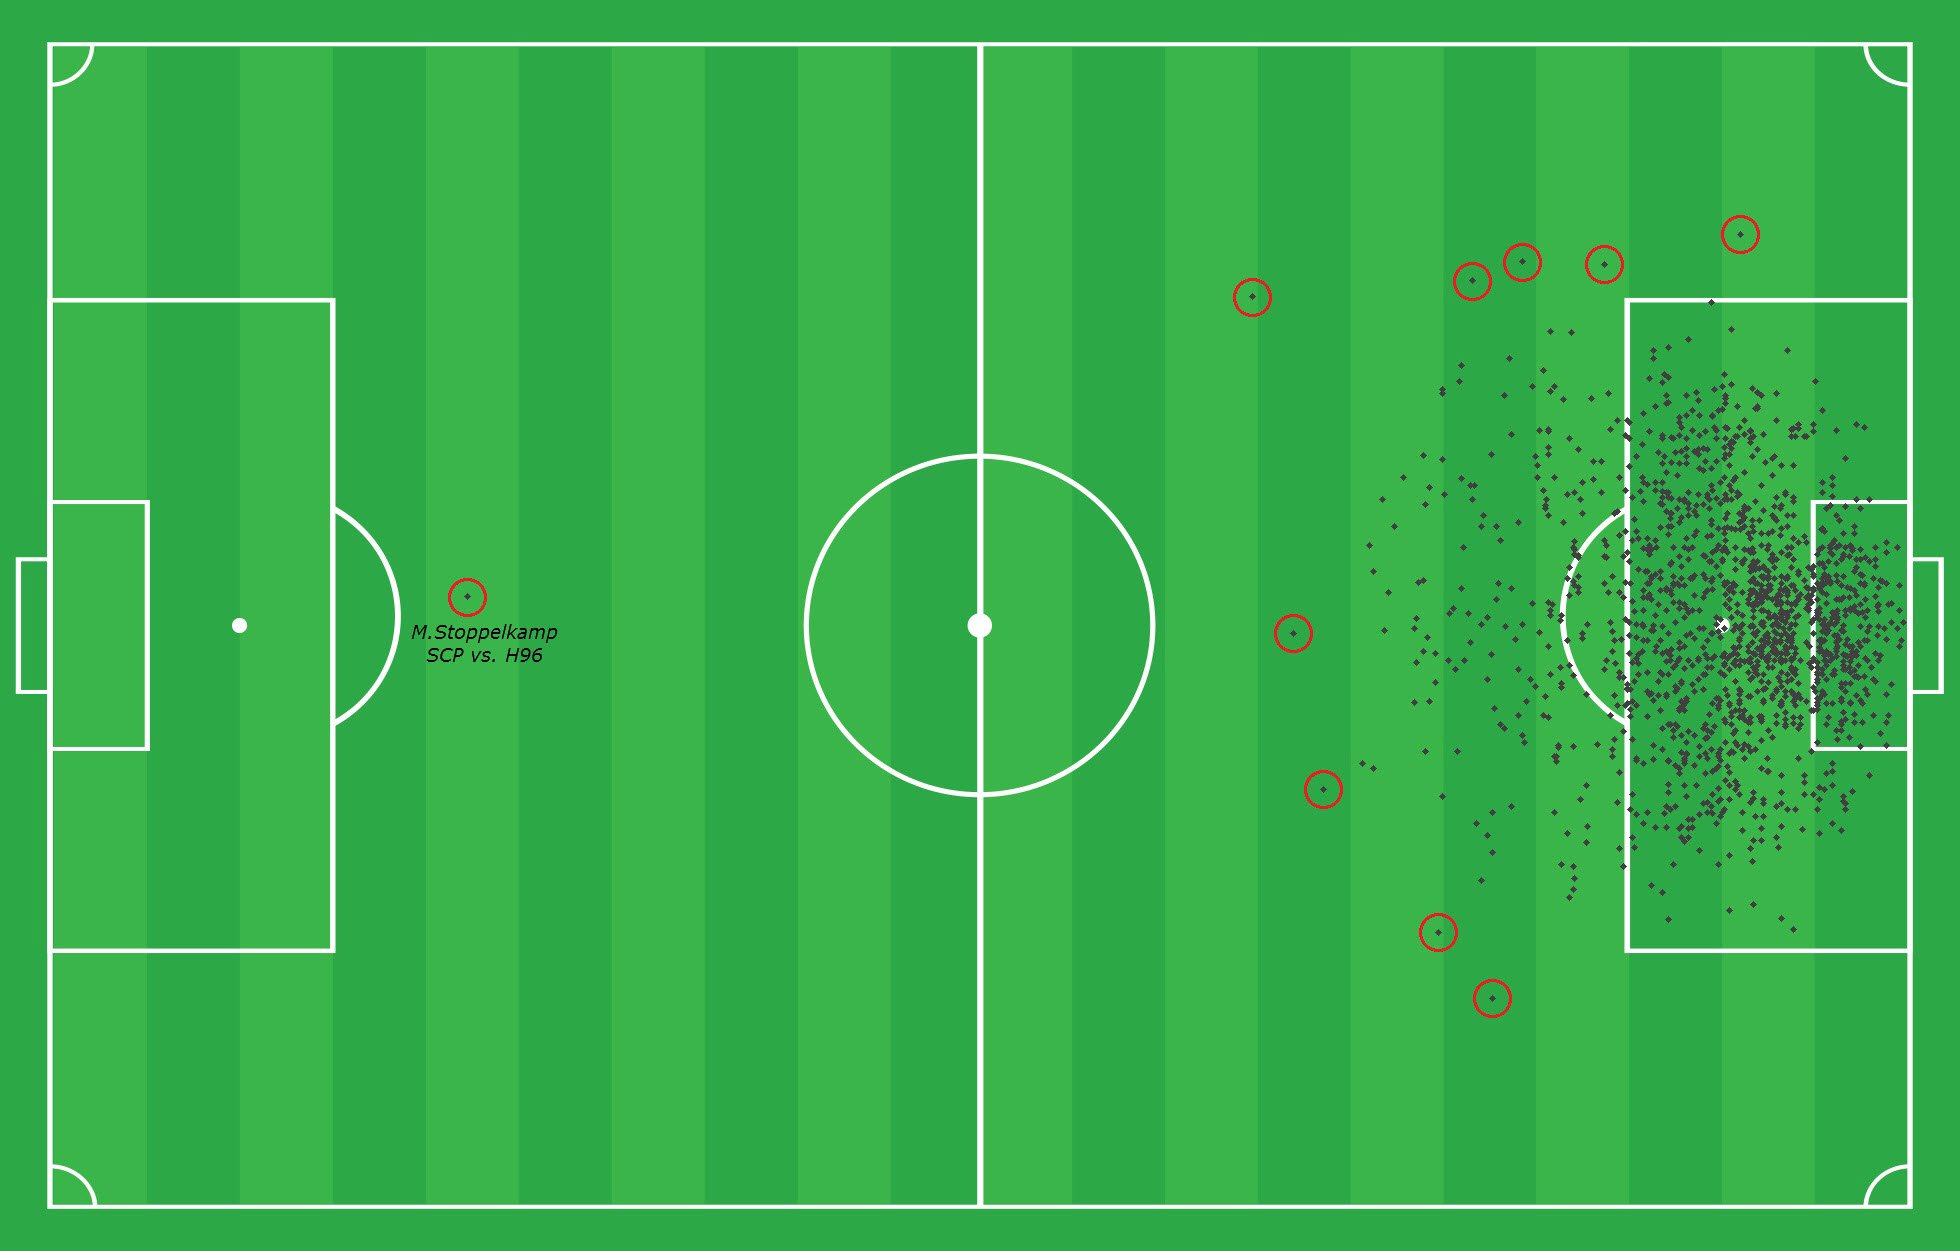
\includegraphics[scale=0.4]{se-wa-jpg/outlier_shots}
\caption[Darstellung der Ausreißer bei Torerfolgen]{Darstellung der Ausreißer bei Torerfolgen}
\label{outlier_shots}
\end{sidewaysfigure}

%\begin{figure}
%\centering
%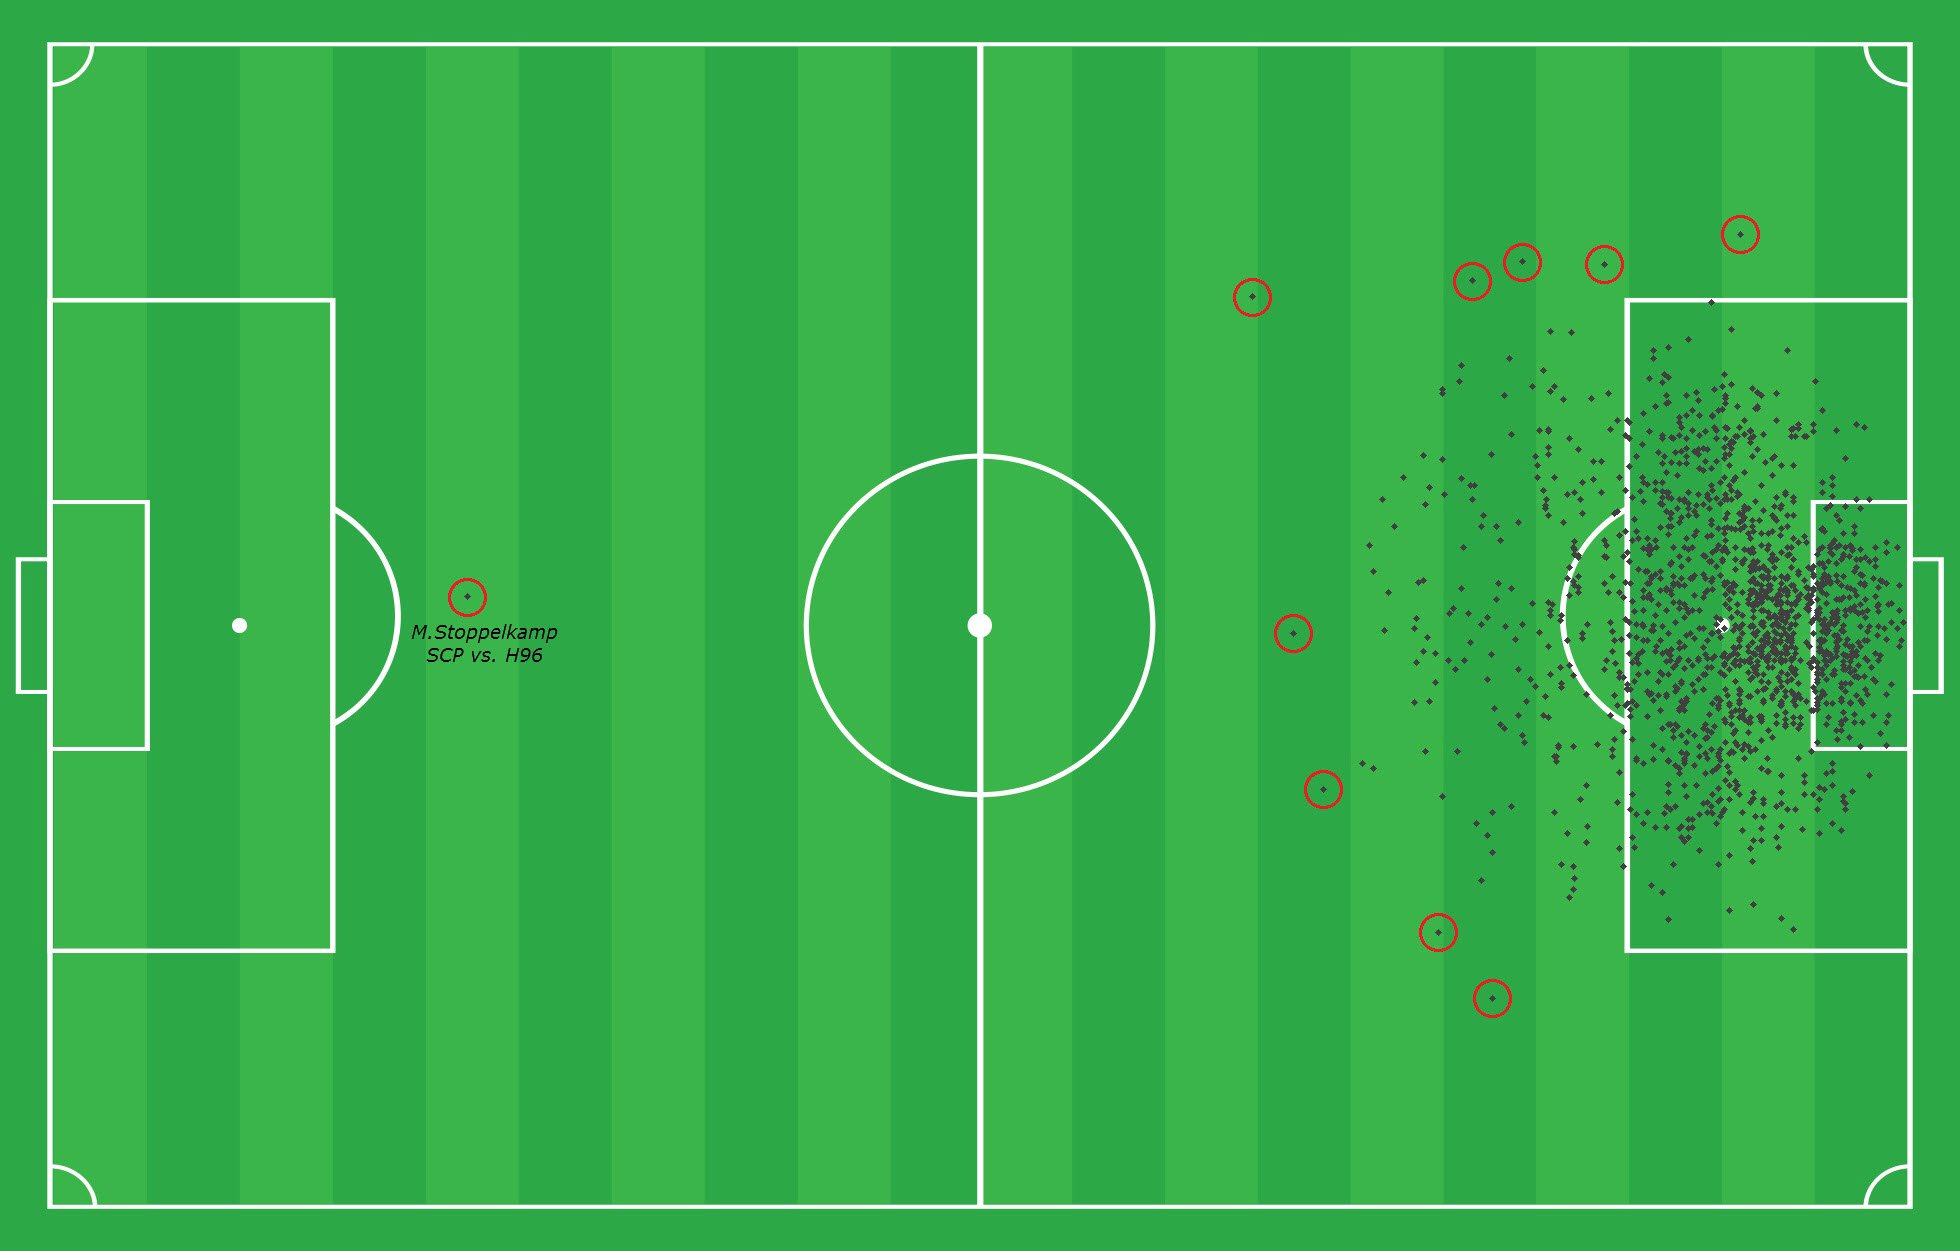
\includegraphics[scale=0.28]{se-wa-jpg/outlier_shots}
%\caption[Ausreißer bei Torerfolge]{Ausreißer bei Torerfolge}
%\label{outlier_shots}
%\end{figure}
